\clearpage
%%%%%%%%%%%%%%%%%%%%%%%%%%%%%%%%%%%%%%%%%%%%%%%%%%%%%%%%%%%%%%%%%%%%%%%%%%%%%%%
\section{Ray Tracing in One Weekend}
%%%%%%%%%%%%%%%%%%%%%%%%%%%%%%%%%%%%%%%%%%%%%%%%%%%%%%%%%%%%%%%%%%%%%%%%%%%%%%%

\begin{itemize}
    \item this is my take on Marc Andreessen's anti-todo\footnotemark\ list
        concept that i have been doing for years no matter the nature of the 
        project or type of work i am doing (i also maintain a bite-sized 
        version in a series of tiny moleskin)
        \footnotetext{ thanks pmarca!
            \textcolor{blue}{\href{https://pmarchive.com/guide_to_personal_productivity.html}{original
        blog post}} (archived by someone) }
    \item test bib \cite{Shirley2024RTW1}
    \item bib working lets go
    \item now that bib is working, thanks to 
        \textcolor{blue}{\href{https://github.com/petershirley}{Peter Shirley}},
        \textcolor{blue}{\href{https://github.com/trevordblack}{Trevor David Black}}, and
        \textcolor{blue}{\href{https://github.com/hollasch}{Steve Hollasch}}
        for this incredible writeup! \cite{Shirley2024RTW1} (
        \textcolor{DarkGreen}{\href{https://raytracing.github.io/books/RayTracingInOneWeekend.html}{course
        link}})
    \item shoutout to 
        \textcolor{blue}{\href{https://x.com/ludwigABAP}{@ludwigABAP}}
        for poasting this course (shoutout ml btw (for you page))
    \item this is my very first c or cpp project (op says it's c flavored cpp) 
        beyond hello worlds and basic basic robotics stuff
    \item i love rust but i am not cracked at all so i would probably not be
        able to follow along in rust
    \item i will, however, follow op's advice to not copy pasta (besides most of 
        makefile compiler flags hehehe) and build it up slowly by typing along
    \item going to try my best to thug this out by Sunday
    \item important setup for fresh arch install (not in order, and just off the
        dome, i likely am forgetting tons of things)
        \begin{itemize}
            \item install unzip (will need for nvim clangd Mason lsp stuff)
            \item install cmake, clangd, gcc stuff
            \item setup debugger for nvim using dap, dap-ui, etc. 
            \item \textbf{build, compile, run:} (i think lol)
                \begin{enumerate}
                    \item \texttt{cmake -B build/Debug -DCMAKE_BUILD_TYPE=Debug} 
                    \item \texttt{cmake --build build/Debug} 
                    \item \texttt{build/rayTracing > image.ppm} 
                \end{enumerate}
        \end{itemize}
    \item op claims that if we can build project correctly in the beginning,
        then we are golden for rest of tutorial
    \item the provided cmake file is cash money and really easy to get working 
        with my setup
        (Figure~\ref{fig:rt_weekend_main_build_success})
        \begin{figure}[ht]
            \centering
            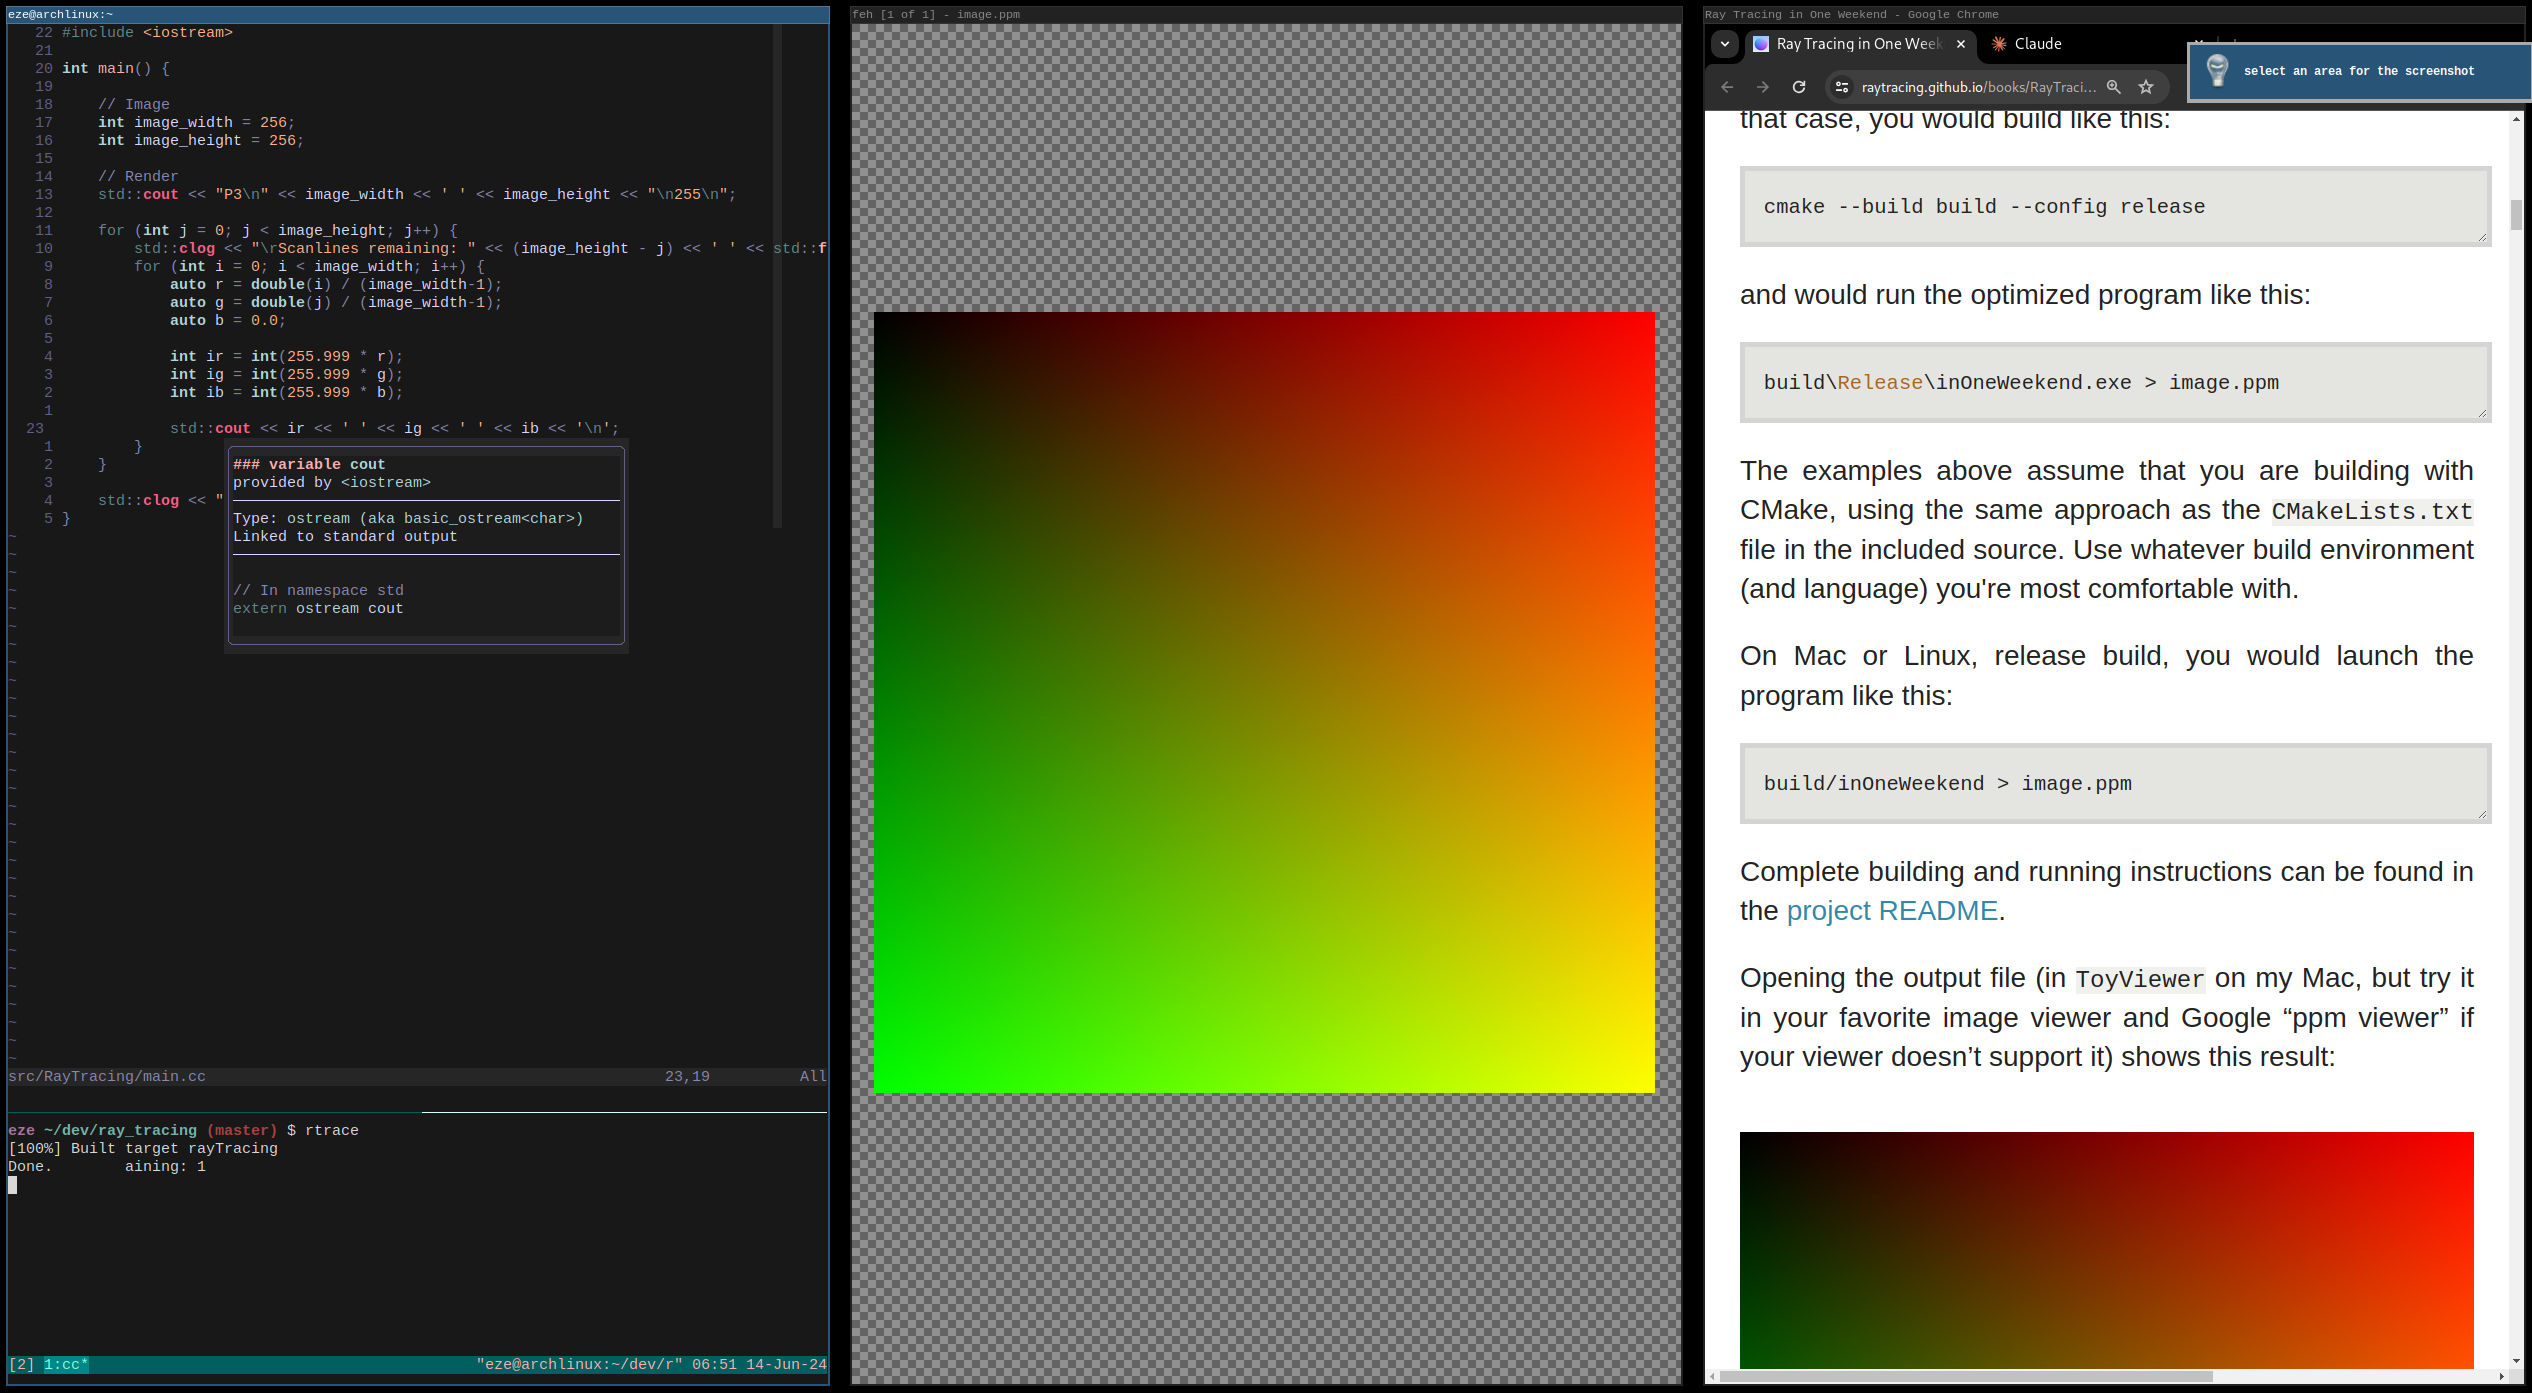
\includegraphics[width=12cm]{rt_weekend_main_build_success}
            \captionsetup{labelfont=bf, textfont=it}
            \caption{build test}
            \label{fig:rt_weekend_main_build_success}
        \end{figure}
    \item make \texttt{rtrace} aliase for build, compile, run, then open image
        in feh, probably terrible idea but whatever 
    \item got color header file with a \texttt{write_color} util function
    \item now working on a \texttt{ray} class which will use our \texttt{vec3} 
        class.
    \item refresher on rays: think of them as functions 
        (Equation~\ref{eq:rays}):

        \begin{equation}
            \mathbf{P}(t) = \mathbf{A} + t\mathbf{b}
            \label{eq:rays}
        \end{equation}

    \item here $\mathbf{P}$ is a 3D position along a line in 3D. $\mathbf{A}$ is
        the ray origin and $\mathbf{b}$ is the ray direction. The ray parameter
        $t$ is a real number (\texttt{double} in the code). Plug in a different
        $t$ and $\mathbf{P}(t)$ moves the point along the ray. Add in negative t
        values and you can go anywhere on the 3D line. For positive $t$, you get
        only the parts in front of $\mathbf{A}$, and this is what is often
        called a half-line or a ray. (Figure~\ref{fig:linear_interpolation}) 
        \begin{figure}[ht]
            \centering
            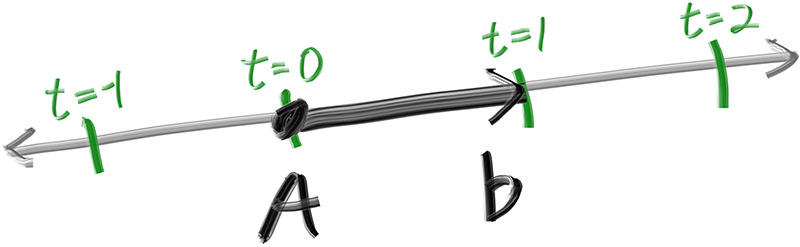
\includegraphics[width=7cm]{linear_interpolation}
            \captionsetup{labelfont=bf, textfont=it}
            \caption{linear interpolation}
            \label{fig:linear_interpolation}
        \end{figure}
    \item to make the actual ray tracer we will make simple camera with 16:9
        aspect ratio since it will be easier to debug $x$ and $y$ 
        transpositions.
    \item we need the height to be at least 1 since we divide width by height
        since it's easier to set the aspect ratio to width then divide by
        height. e.g. $width/height = 16/9 = 1.7778$
    \item apparently this is just an \textit{optimistic} (my words) ratio since 
        these values are not integers. we approximate the aspect ratio as best 
        we can by rounding height to the nearest integer (and don't allow it 
        to be less than one)
    \clearpage
    \item now we have a camera center in 3d space from which all the rays will
        originate (commonly referred to as the \textit{eye point}). we initially
        set the distance between the viewport of the camera center point to be
        one unit. This is often referred to as the \textit{focal length}.
    \item we will use \textit{right-handed coordinates} (right hand rule gang)
        Figure~\ref{fig:camera_rh_rule}
    \begin{figure}[ht]
        \centering
        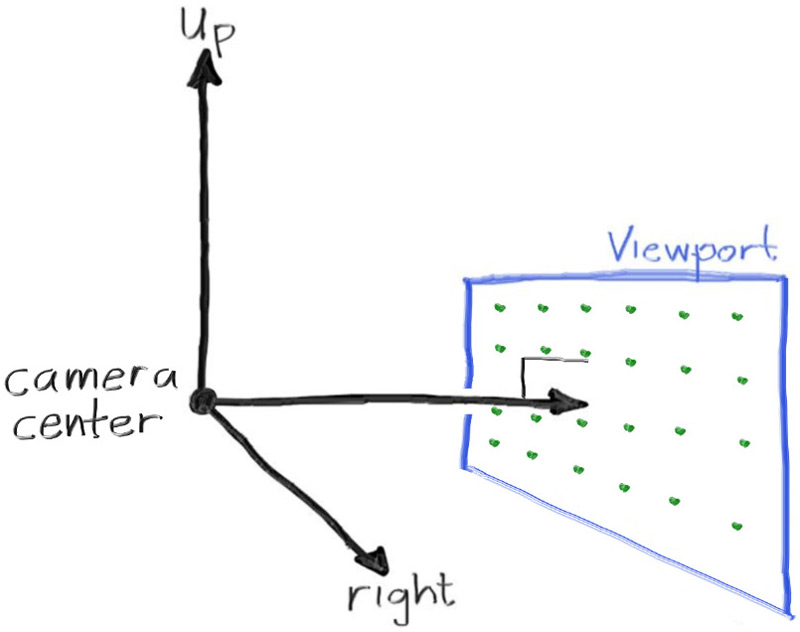
\includegraphics[width=9cm]{camera_rh_rule}
        \captionsetup{labelfont=bf, textfont=it}
        \caption{camera geometry}
        \label{fig:camera_rh_rule}
    \end{figure}
    \item unfortunately, the camera pose conflicts with the way we would like to
        render our image starting from the upper left pixel row by row scanning
        across from left to right. (Figure~\ref{fig:image_coord_system})
        \begin{figure}[ht]
            \centering
            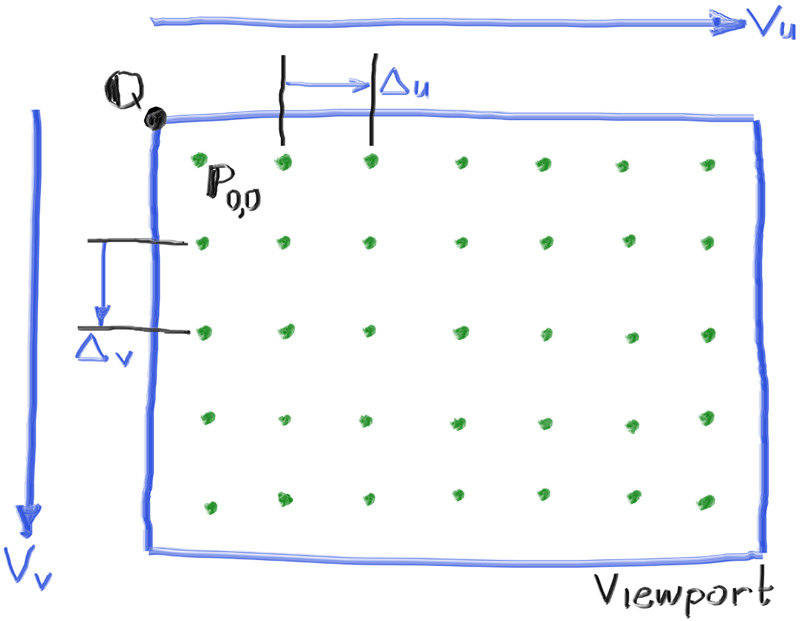
\includegraphics[width=9cm]{image_coord_system}
            \captionsetup{labelfont=bf, textfont=it}
            \caption{viewport and pixel grid}
            \label{fig:image_coord_system}
        \end{figure}
    \item we have example 7x5 resolution image, the viewport upper left corner
        $\mathbf{Q}$, the pixel $\mathbf{P_{0,0}}$ location, the viewport vector
        $\mathbf{V_{u}}$ (viewport_u), the viewport vector $\mathbf{V_{v}}$
        (viewport_v), and the pixel delta vectors $\mathbf{\Delta u}$ and 
        $\mathbf{\Delta v}$.
    \item now we add a simple gradient to the \texttt{ray_color} function which
        will linearly blend white and blue depending on the height of $y$
        coordinate $after$ scaling the ray direction to unit length. op uses
        standard graphics trick to linearly scale $0.0 \leq a \leq 1.0$. when
        $a=1.0$, i want blue, when $a=0.0$, i want white. in between, i want a
        blend. here's a \textit{linear interpolation} or \textit{linear
        interpolation}; commonly reffered to as a \textit{lerp} between two
        values. a lerp is always of the form 

        \begin{equation}
            blendedValue = (1-a)\cdot startValue + a \cdot endValue
        \end{equation}

        with $a$ going from zero to one (ayy lmao).
    \item now it's time to add a sphere (folks use spheres in ray tracers
        because calculating whether a ray hits a sphere is relatively simple.
    \item the equation for a radius $r$ that is centered at the origin is an
        important mathematical equation

        \begin{equation}
            x^{2}+y^{2}+z^{2}
        \end{equation}

    \item this of this as saying that if a given point $(x,y,z)$ is on the
        surface of the sphere, then $x^{2}+y^{2}+z^{2}=r^{2}$. if a given point
        $(x,y,z)$ is \textit{inside} the sphere, then $x^{2}+y^{2}+z^{2}<r^{2}$,
        and if a given point $(x,y,z)$ is \textit{outside} the sphere, then
        $x^{2}+y^{2}+z^{2}>r^{2}$.
    \item if we want to allow the sphere center to be at an arbitrary point 
        $(C_{x},C_{y},C_{z})$, then the equation is not so nice:

        \begin{equation}
            (C_{x} - x)^{2}+(C_{y} - y)^{2}+(C_{z} - z)^{2} = r^{2}
        \end{equation}

    \item in graphics, you almost always want formulas to be in terms of
        vectors so we don't need to write out so many terms.
    \item note that the vector from point $\mathbf{P}=(x,y,z)$ to center
        $\mathbf{C}=(C_{x},C_{y},C_{z})$ is $(\mathbf{C}-\mathbf{P})$
    \item we can ust the definition of the dot product:

        \begin{equation}
            (\mathbf{C}-\mathbf{P}) \cdot (\mathbf{C}-\mathbf{P}) = (C_{x} - x)^{2}+(C_{y} - y)^{2}+(C_{z} - z)^{2} = r^{2}
        \end{equation}

    \item then we can rewrite the equation of the sphere in vector form as:

        \begin{equation}
            (\mathbf{C}-\mathbf{P}) \cdot (\mathbf{C}-\mathbf{P}) = r^{2}
        \end{equation}

    \item we can read this as ``any point $\mathbf{P}$ that satisfies this
        equation is on the sphere". we want to know if our ray 
        $\mathbf{P}(t)=\mathbf{Q}+t\mathbf{d}$ ever hits the sphere anywhere. if
        it does hit the sphere, there is some $t$ for which $\mathbf{P}(t)$
        satisfies the sphere equation. So we are looking for any $t$ where this
        is true:

        \begin{equation}
            (\mathbf{C}-\mathbf{P}(t)) \cdot (\mathbf{C}-\mathbf{P}(t)) = r^{2}
        \end{equation}

    \item which can be found by replacing $\mathbf{P}(t)$ with its expanded
        form:

        \begin{equation}
            (\mathbf{C}-(\mathbf{Q}+t\mathbf{d})) \cdot
            (\mathbf{C}-(\mathbf{Q}+t\mathbf{d})) = r^{2}
        \end{equation}

    \item we have three vecs on the left dotted by three vecs on right, if we
        solved for the full dot product we would get nine vectors (slop), we
        need to solve for t with quadratic equation, so first shape equation
        above into quadratic by first isolating $t$ terms, then distribute dot
        product, then move $r^{2}$ to left hand side:

    \item boom
        \begin{equation}
            (-t\mathbf{d}+(\mathbf{C}-\mathbf{Q})) \cdot
            (-t\mathbf{d}+(\mathbf{C}-\mathbf{Q})) = r^{2}
        \end{equation}

    \item bop
        \begin{equation}
            t^{2}\mathbf{d}\cdot \mathbf{d} - 2t\mathbf{d} \cdot
            (\mathbf{C}-\mathbf{Q}) + (\mathbf{C}-\mathbf{Q}) \cdot
            (\mathbf{C}-\mathbf{Q}) = r^{2}
        \end{equation}

    \item pow
        \begin{equation}
            t^{2}\mathbf{d}\cdot \mathbf{d} - 2t\mathbf{d} \cdot
            (\mathbf{C}-\mathbf{Q}) + (\mathbf{C}-\mathbf{Q}) \cdot
            (\mathbf{C}-\mathbf{Q}) - r^{2} = 0
        \end{equation}

    \item we can now run quadratic formula on this bad boy and all the vecs are
        reduced to scalars by dot prod.

        \begin{equation}
            \frac{-b\pm \sqrt{b^{2}-4ac}}{2a}
        \end{equation}

    \item can now for $t$ using the terms $a, b,$ and $c$:

        \begin{equation}
            a = \mathbf{d}\cdot \mathbf{d}
        \end{equation}

        \begin{equation}
            b = -2\mathbf{d}\cdot (\mathbf{C}-\mathbf{C})
        \end{equation}

        \begin{equation}
            c = (\mathbf{C}-\mathbf{Q}) \cdot (\mathbf{C}-\mathbf{Q}) - r^{2}
        \end{equation}
    \item this will yield either positive (2 real solutions), negative (no real
        solutions) or zero (1 real solution)

        \clearpage

    \item the algebra almost always relates very directly to the geometry 
        (Figure~\ref{fig:ray_sphere_intersection_roots})
        \begin{figure}[ht]
            \centering
            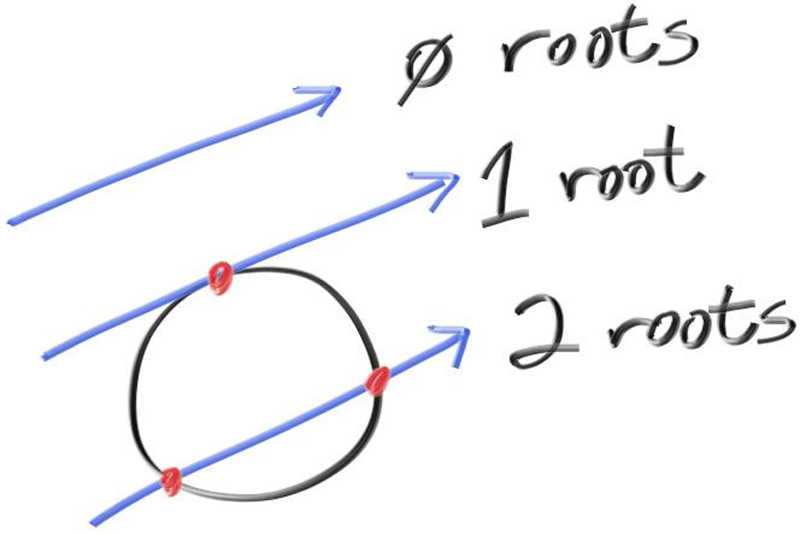
\includegraphics[width=7cm]{ray_sphere_intersection_roots}
            \captionsetup{labelfont=bf, textfont=it}
            \caption{ray sphere intersection roots}
            \label{fig:ray_sphere_intersection_roots}
        \end{figure}
    \item create first ray traced image by placing a small sphere at -1 on the
        z-axis and then coloring red any pixel that intersects it.
        (Figure~\ref{fig:red_ray_trace_sphere})
        \begin{figure}[ht]
            \centering
            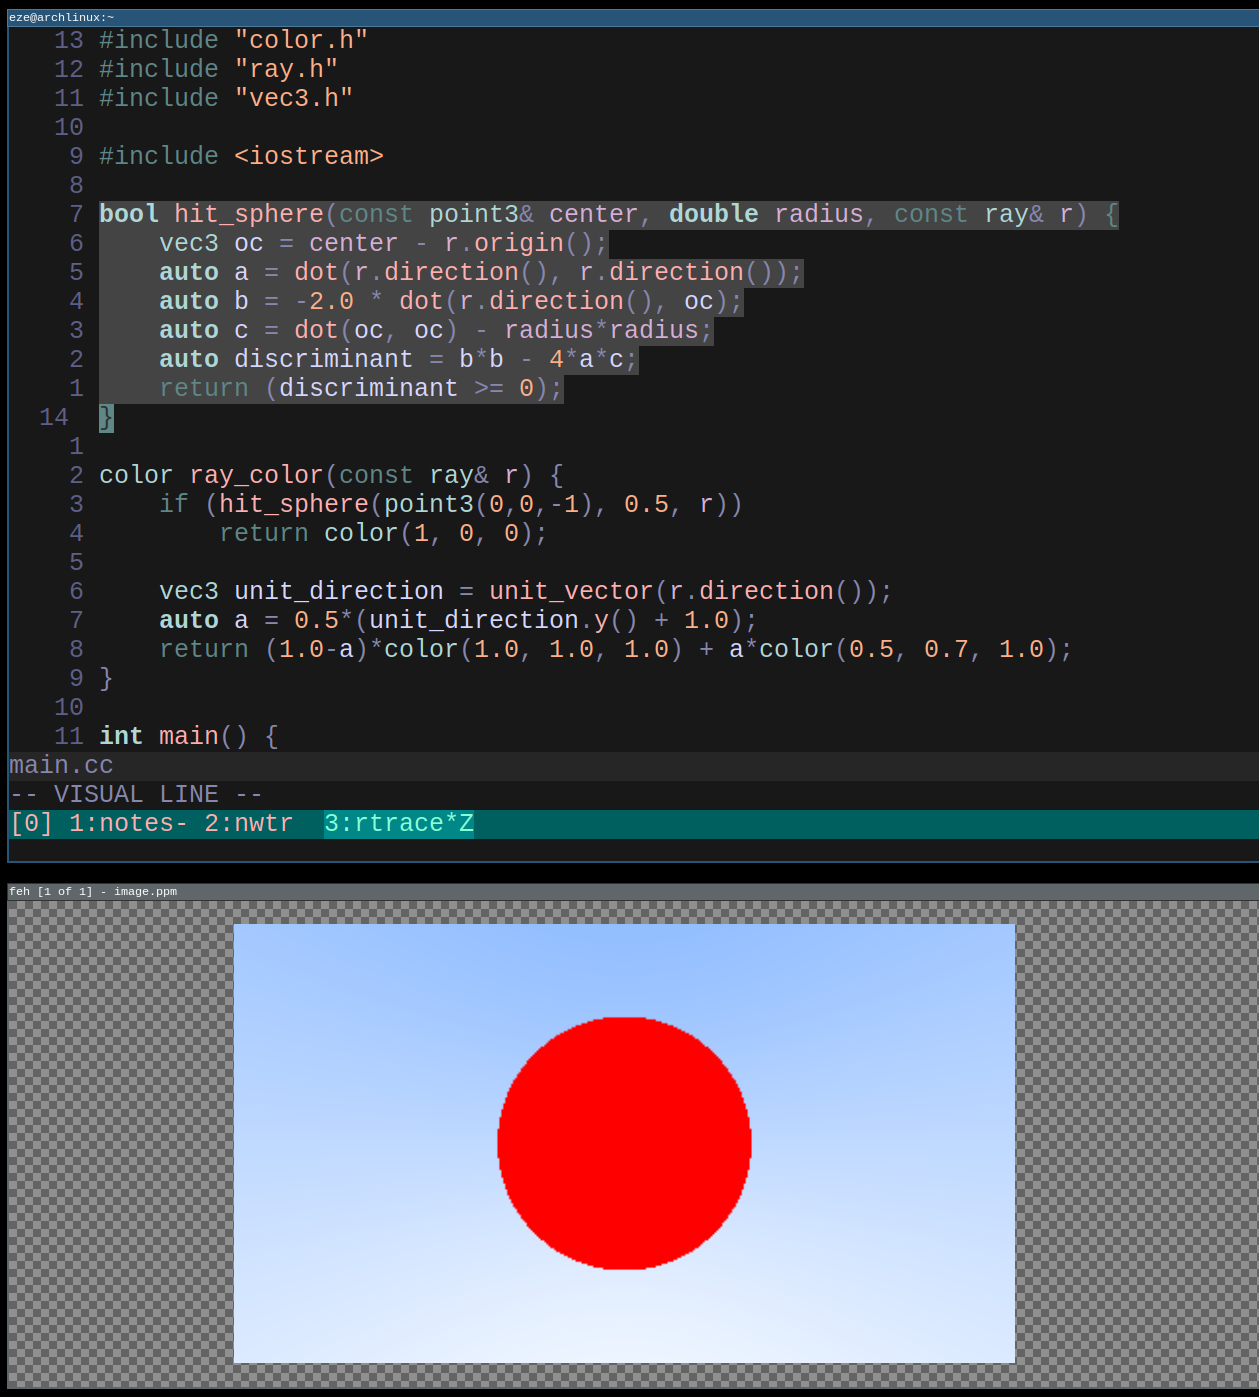
\includegraphics[width=12cm]{red_ray_trace_sphere}
            \captionsetup{labelfont=bf, textfont=it}
            \caption{simple red sphere}
            \label{fig:red_ray_trace_sphere}
        \end{figure}
    \item this lacks all sorts like shading, reflection rays, and more than a
        single object, also this solution doesn't account for the camera really
        since it will also work with the sphere center at +1 (behind camera)
        \clearpage
    \item i should start writing section titles... maybe later %todo
    \item shading with surface normals, a normal is just perpendicular to the
        surface at the point of intersection.
    \item we have key design decision to make for normal vectors in code:
        whether normal vecs will have arbitrary length, or should we normalize?
        \textit{much to think about...}
    \item it is tempting to skip the expensive sqrt op involved in normalizing
        the vector, in case it's not needed. in practice, however, there are
        three important observations. first, if a unit-length normal vector is
        \textit{ever} required, then you might as well do it up from once,
        instead of over and over again ``just in case" for every location where
        unit-length is required. Second, we \textit{do} require unit-length
        normal vecors in several places. Third, if you require normal vectors to
        be unit length, then you can often efficiently generate that vec with an
        understanding of the specific geometry class, in its consructor, or in
        the \texttt{hit()} function. e.g., sphere normals can be made unit
        length simply by dividing by the sphere radius, avoiding the sqrt
        entirely.
    \item unit length sphere normals will be used up front for these reasons
    \item the outward normal for a sphere is in the direction of the hit point
        minus the center (Figure~\ref{fig:sphere_normal_direction})
        \begin{figure}[ht]
            \centering
            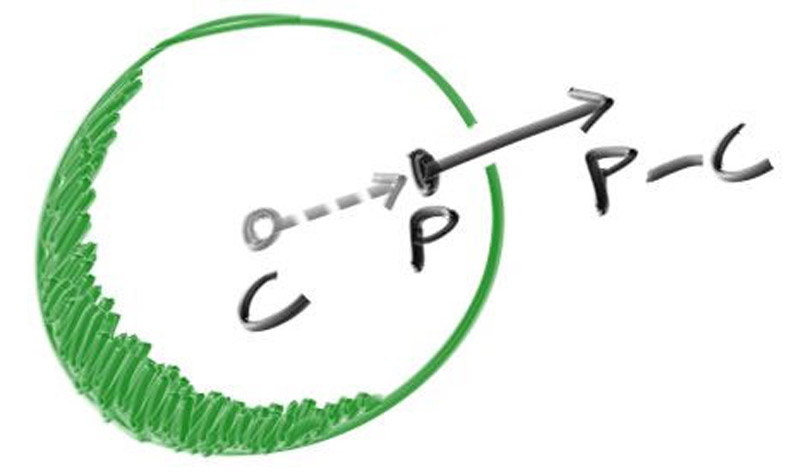
\includegraphics[width=12cm]{sphere_normal_direction}
            \captionsetup{labelfont=bf, textfont=it}
            \caption{sphere surface-normal geometry}
            \label{fig:sphere_normal_direction}
        \end{figure}
    \item we don't have light let so let's use a common trick for visualizing
        normals: a color map. we can assume $\mathbf{n}$ is a unit length vec,
        so each component is between -1 and 1; we just map eacho component to
        the interval fro m0 to 1, and then map $(x,y,z)$ to $(red,green,blue)$.
        for the normal, we need the hit point, not just whether we hit or not
        (which is all we are doing currently:
        Figure~\ref{fig:red_ray_trace_sphere}). we only have 1 sphere in the
        schene and it's right in front of the camera, so we won't worry about
        negative values of $t$ yet. We'll just assume the closest hit point
        (smallest $t$) is the one that we want. These changes in the code let us
        compute and visualize $\mathbf{n}$.
\end{itemize}
